% !TEX root = ../Thesis.tex
% !TEX spellcheck = en-US

\chapter{GNS3}
\label{ch:gns3}

GNS3, whose original title was ``Graphical Network Simulator-3,'' is a software project, comprising several distinct components and, despite the ``simulator'' in its name, \emph{as a whole}, it falls under the category that, in this thesis, is called \emph{emulator}. % TODO try to (either with a source, or speculating) relate the name with ns-3
% TODO also: cite the source for the name
By ``as a whole,'' it is meant that, as shall be seen later, although some of its components, like the Dynamips program, are emulators in a strict sense---i.e. its purposes is to run real machine code on a different hardware architecture (than its native one)---, it differentiates itself, on a high-level perspective, from a simulator which is a program designed to execute a mathematical model, processing modeled events as internal data-structures with a collection of preset algorithms that somehow mimic (a part of) the reality.

It's important to notice that a necessary step towards the goal of this this thesis is to systematize a technical description of the architecture and functional underpinnings of the GNS3 system, how is it executed, how does it interact with the hardware and software it is running in, how much resources does it take to work with GNS3 according to the \emph{mode} it is running in, etc., as that is an aspect that is yet to be further explored for, at least, the following reasons:  % TODO improve the writing how is etc written in Engilsh?
for one, the consulted academic material (i.e. research papers, mostly) is very brief and omissive in regards to the design, architecture and implementation of GNS3, and so is the official website and documentation. Besides that, many interesting details are in the ``paraofficial'' videos available via YouTube, but certified as official, by David Bomball, namely a comprehensive overview of the architecture (compared with the functionality) of GNS3 by its creator, Jeremy Grossmann, and essentially are not anywhere else, at least from authoritative sources. % TODO same as the previous "sentence". Cite the videos (how and which ones?). How's the name of DB spelled?

% TODO add a figure (a screen shot) showing the "official" submitter of GNS3 videos (and maybe the channel and/or links from the gns3 official website)

% end of intro

\section{GNS3's purpose and \emph{raison d'être}}
\label{sec:gns3why}

The GNS3 project was created by Jeremy Grossmann at the University. % TODO find out which one was it?
It was built with a main goal: allowing students of Cisco certifcations to be able to test network topologies and practice their skills with the same software stack that is used in real Cisco devices and the hosts connected to them---from the operating system, up until application--level network utilities---, without having to use the expensive official solutions for that, or having to fall back on the limited graphical simulators like Cisco's Packet Tracer. % TODO how can we know if this was really the goal and cite

Despite still having a strong relation with training for Cisco CCNA and related certifications, the magnitude of the project, part of which comes from an inherent extensibility, has made it suitable for a myriad of use-cases, of which testing and configuring topologies in the context of the modern \emph{DevOps}-driven infrastructure setup and implementation is a good example.
But also potential applications that are still relatively unexplored.
Such is the case of its usage in academic teaching and learning, the goal of of this work.

% end of section gns3why

\section{Building blocks. The programs ``inside'' GNS3}
\label{sec:gns3buildingblocks}

Here's a cool table that I made where I have put systematic information about the repositories and stuff like that.

\begin{table}
  \centering
  \small
  \begin{tabulary}{0.8\textwidth}{lLL}
    \toprule
      \textbf{Part}  & \textbf{Role}                                                       & \textbf{Source code repository}\\
    \midrule
      GNS3 GUI       & A desktop application that runs on a graphical OS                   & \scriptsize\url{https://github.com/GNS3/gns3-gui}\\
      Dynamips       & A MIPS emulator, used by the \emph{backend} to run (old) IOS images & \scriptsize\url{https://github.com/GNS3/dynamips}\\
    \bottomrule
  \end{tabulary}
  \caption{%
    Intrinsic parts of GNS3, constituting separate and independent codebases
  }
  \label{tab:gns3components}
\end{table}


\subsection{GNS3 GUI}
\label{subsec:gns3gui}

Interaction between the end-user and GNS3 is usually---though, as will be clear, not necessarily---made in a graphical environment.
A GNS3 project, called a \emph{topology}, is constantly opened on one single window (per running instance of the application) and is graphically represented in the main section of the window.

\begin{figure}
  \centering
  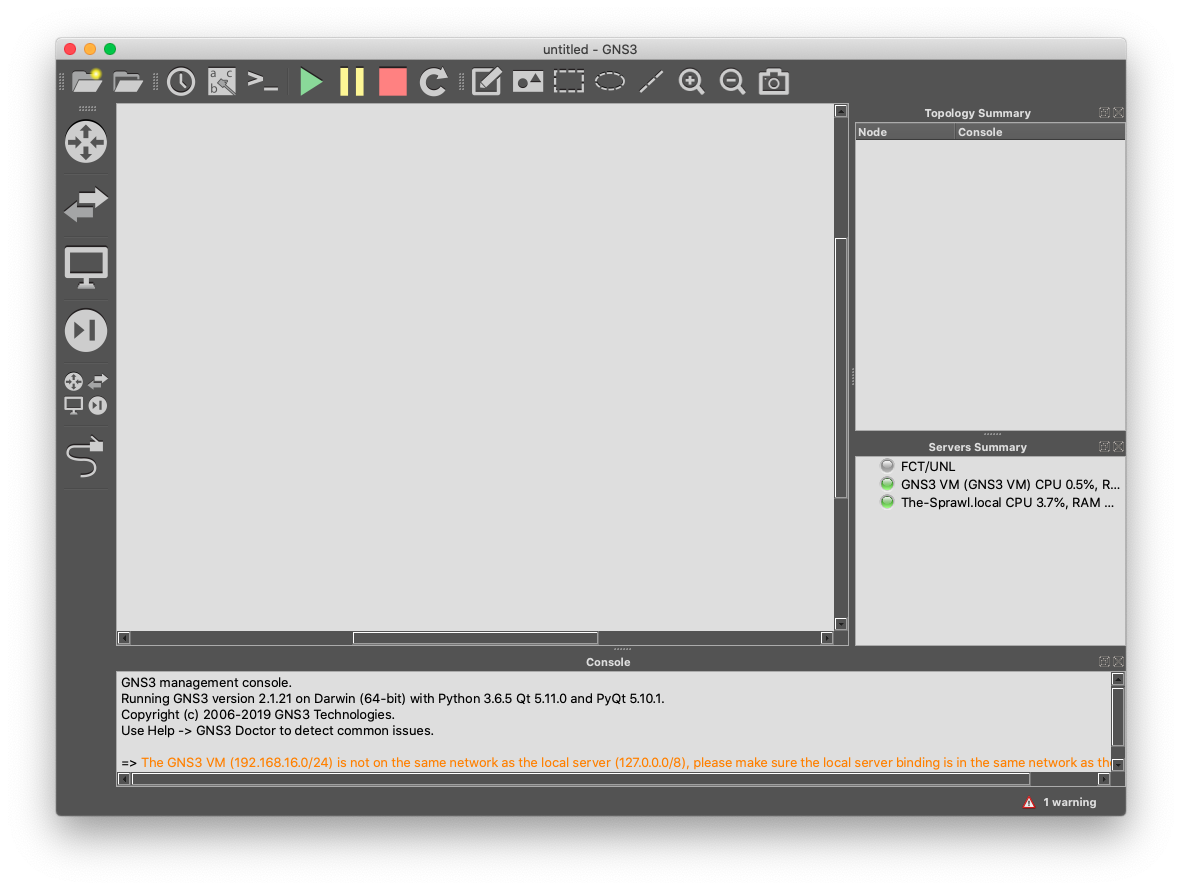
\includegraphics[width=0.8\textwidth]{gns3empty}
  \caption{An empty GNS3 topology shown in the GUI}
\end{figure}

\subsection{Dynamips}
\label{subsec:gns3dynamips}

The Dynamips emulator is a standalone \emph{free} program, written in C, that, normally, comes distributed together with the whole GNS3 package.
It is an emulator for a MIPS processor and was the original--single way to run the software of the Cisco nodes of the topologies created with GNS3.

% end of section gns3buildingblocks

\section{General architecture}
\label{sec:gns3architecture}

% end of section gns3architecture

\section{GNS3 in action}
\label{sec:gns3inaction}

% end of section gns3inaction

\section{Performance and resources considerations}
\label{sec:gns3performance}

% end of section gns3performance

% end of chapter
